\section{Results}
\label{SECIV}\label{sec:results}

\begin{itemize}
\item 1 day of simulated $h(t)$.
\item $h(t)$ has power spectrum \sout{prescribed for ``zero detuning, high power'' model in \cite{Shoemaker:2009p9770}} that somewhat resembles initial \textsc{ligo} noise models
\item $h(t)$ generated by passing white, Gaussian noise through a bank of \textsc{iir} filters
\item 1 noninjections run
\item 10 injections runs
\item injections are distributed uniformly in log distance, uniformly in sky location and binary orientation
\item injections are reweighted to be uniformly distributed in volume
\item injections are 80$\pm$20 seconds apart
\item there are $\approx$ 10k injections
\end{itemize}

\begin{figure}[htbp]
\begin{center}
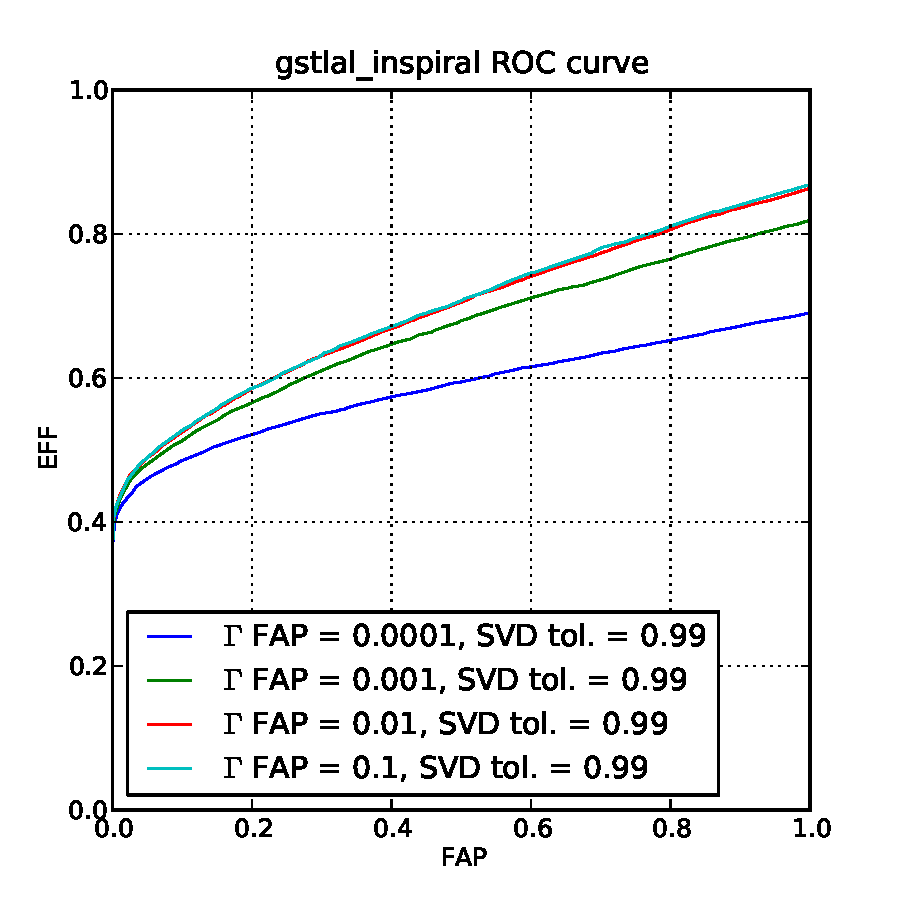
\includegraphics[scale=0.4]{figures/roc_99.pdf}
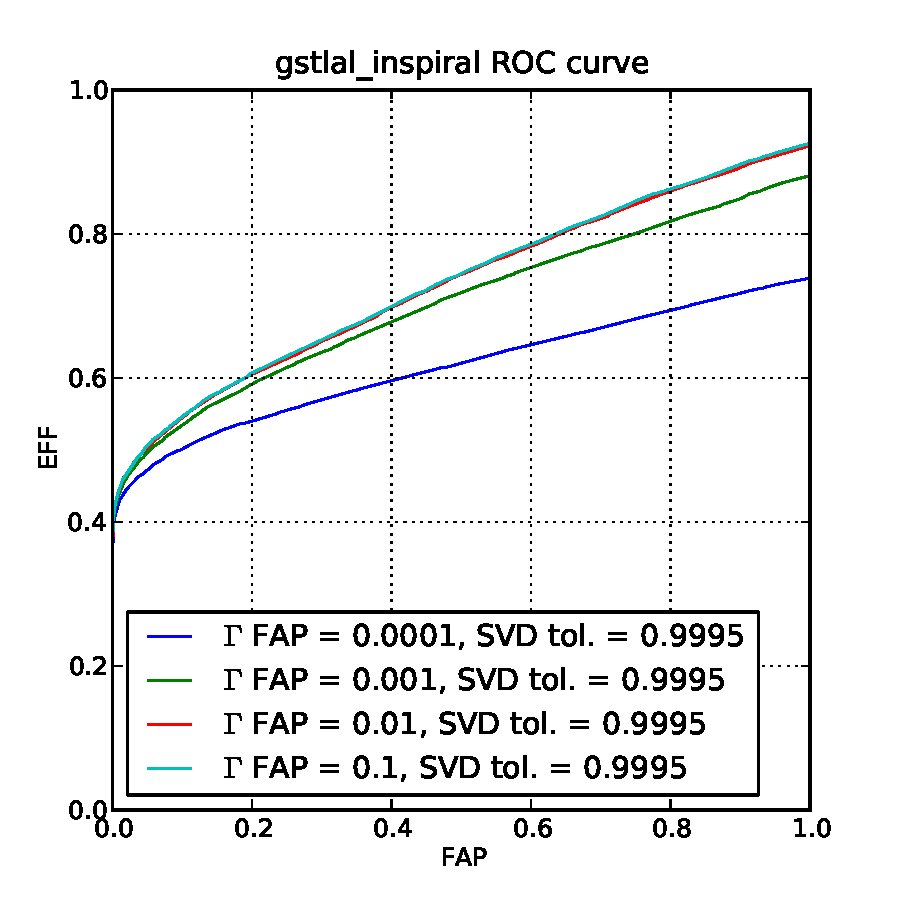
\includegraphics[scale=0.4]{figures/roc_9995.pdf}
\caption{Receiver operating characteristic (\textsc{roc}) curve of detection efficiency (\textsc{eff}) versus false alarm probability (\textsc{fap}).}
\label{fig:roc}
\end{center}
\end{figure}
